%!TEX root = report.tex

\subsection{Performance Measure}
The performance of the localization can be quantified by the distance from the calculated target point to its real position (measured with a laser pointer). 
Both algorithms, fixed-height and free-height (see § \ref{sec:triangulation}), are applied. The errors in the x-y plane for fixed-height and free-height as well as the 3D error for free-height are considered. 

With the four available cameras there are several camera combinations that can be used for the calculation.
It was found that the error in the position of the robot is highly dependent on which cameras are used for triangulating the image points. 
Currently, the best camera combination is determined based on the error between the measured and actual position of the robot.
In later experimental setups, however, the real position of the robot will not be directly measured, so it is necessary to find another criterion for evaluating the camera combinations.
One option considered was to use the errors of the reprojection of the reference points, whose positions are already well-known.
The results of this approach, shown in Figure~\ref{fig:res0_err}, however, suggest that the correlation between the reference point error and the robot position error is not strong enough, so a different criterion needs to be found.
This task is beyond the scope of the present project so in the following section, all camera combinations are considered and the real position of the robot is used for measurement of performance.


\begin{figure}[H]
    \centering
    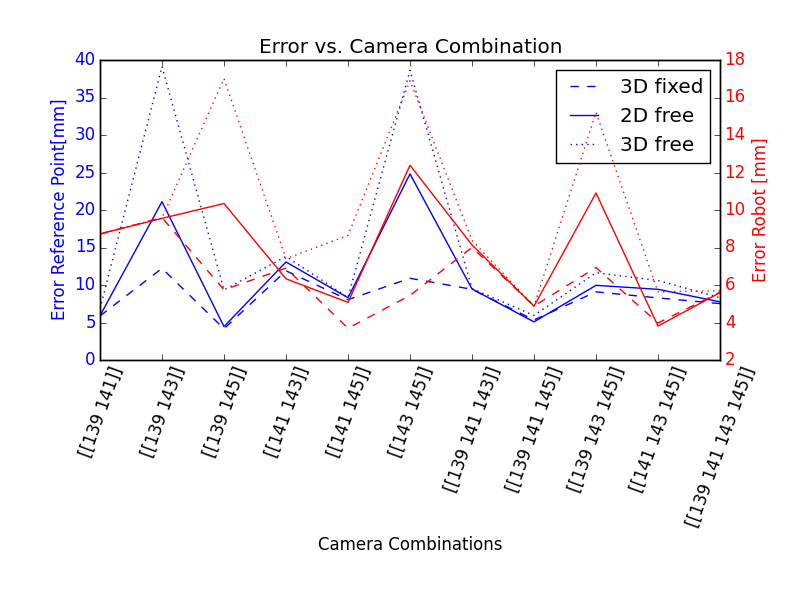
\includegraphics[width=.8\linewidth]{files/res0_combi_4.png}
    \caption{Experiment in Atrium: results of visual localization for various camera combinations.}
    \label{fig:res0_err}
\end{figure}
